%----------------------------------------------------------------------------------------
%	PACKAGES AND THEMES
%----------------------------------------------------------------------------------------

\documentclass{beamer}

\mode<presentation> {
\usetheme{Madrid}

\setbeamertemplate{navigation symbols}{} % To remove the navigation symbols from the bottom of all slides uncomment this line
}

% German Language Settings
\usepackage[utf8]{inputenc}
\usepackage[ngerman]{babel}

\usepackage{graphicx} % Allows including images
\usepackage{booktabs} % Allows the use of \toprule, \midrule and \bottomrule in tables
\usepackage{hyperref} % For Table of Content in PDF
\usepackage{multirow}



\newcommand{\backupbegin}{
   \newcounter{finalframe}
   \setcounter{finalframe}{\value{framenumber}}
}
\newcommand{\backupend}{
   \setcounter{framenumber}{\value{finalframe}}
}

%----------------------------------------------------------------------------------------
%	TITLE PAGE
%----------------------------------------------------------------------------------------

\title[Assignment 5]{Präsentation von Assignment 5} % The short title appears at the bottom of every slide, the full title is only on the title page

\author{Ramil Sabirov, Joel Choi, Eric Remigius} % Your name
\institute[] % Your institution as it will appear on the bottom of every slide, may be shorthand to save space
{
RWTH Aachen \\ % Your institution for the title page
\medskip
\textit{Gruppe3} % Your email address
}
\date{\today} % Date, can be changed to a custom date

\begin{document}

\begin{frame}
\titlepage % Print the title page as the first slide
\end{frame}

%----------------------------------------------------------------------------------------
%	PRESENTATION SLIDES
%----------------------------------------------------------------------------------------

%------------------------------------------------
\section{Task 1}
%------------------------------------------------

\begin{frame}
\frametitle{Zeitschätzung}
\pause
Bis heute:
\begin{enumerate}
\item[•]Nutzung des maximalen Verzweigungsgrades $k_{max}$.
\item[•]Für Tiefe $d$ Zeitaufwand: $t(d) = t_i(d) + t_b(d)$
\item[•]Zeitaufwand für Tiefe $d+1$:
\begin{align*}
t(d+1) =& t_i(d+1) + t_b(d+1) \leq\\ &k_{max} * (t_i(d) + t_b(d)) = k_{max} * t(d)
\end{align*}
\end{enumerate}
$\rightarrow$ Problem: sehr konservative Zeitschätzung, hohes Endzeitkonto.\\\hfill\break
\pause
Ab heute:
\begin{enumerate}
\item[•]Nutzung des \textbf{durchschnittlichen} Verzweigungsgrades.
\item[•]Berücksichtigung des Prunings
\end{enumerate}
\end{frame}

%------------------------------------------------
\section{Task 2}
%------------------------------------------------

\begin{frame}
\frametitle{Suchfenster}
\pause
\textbf{Annahme:} Mit erweiterter Tiefe ändert sich der Stellungswert nur minimal.\\\hfill\break
\pause
Strategie mit Fenstergröße $a$:
\begin{enumerate}
\item[1.] Suche Tiefe 1 \textbf{ohne} Suchfenster.
\item[2.] Tiefe d lieferte Stellungswert $val_d$. Suche Tiefe d+1 mit \textbf{festgesetzten} Intervall $[\alpha, \beta] = [val_d - a, val_d + a]$
\end{enumerate}
\hfill\break
Wegen festgesetztem Intervall, kann der eigentliche Stellungswert verfehlt werden.
$\rightarrow$ Neusuche notwendig!\\
\pause
\hfill\break
Hoffnung: Festgesetztes Intervall hilft mehr Teilbäume abzuschneiden.
\end{frame}



%------------------------------------------------
\section{Task 3}
%------------------------------------------------

\begin{frame}
\frametitle{Suchfenster Statistiken}
  \begin{figure}
    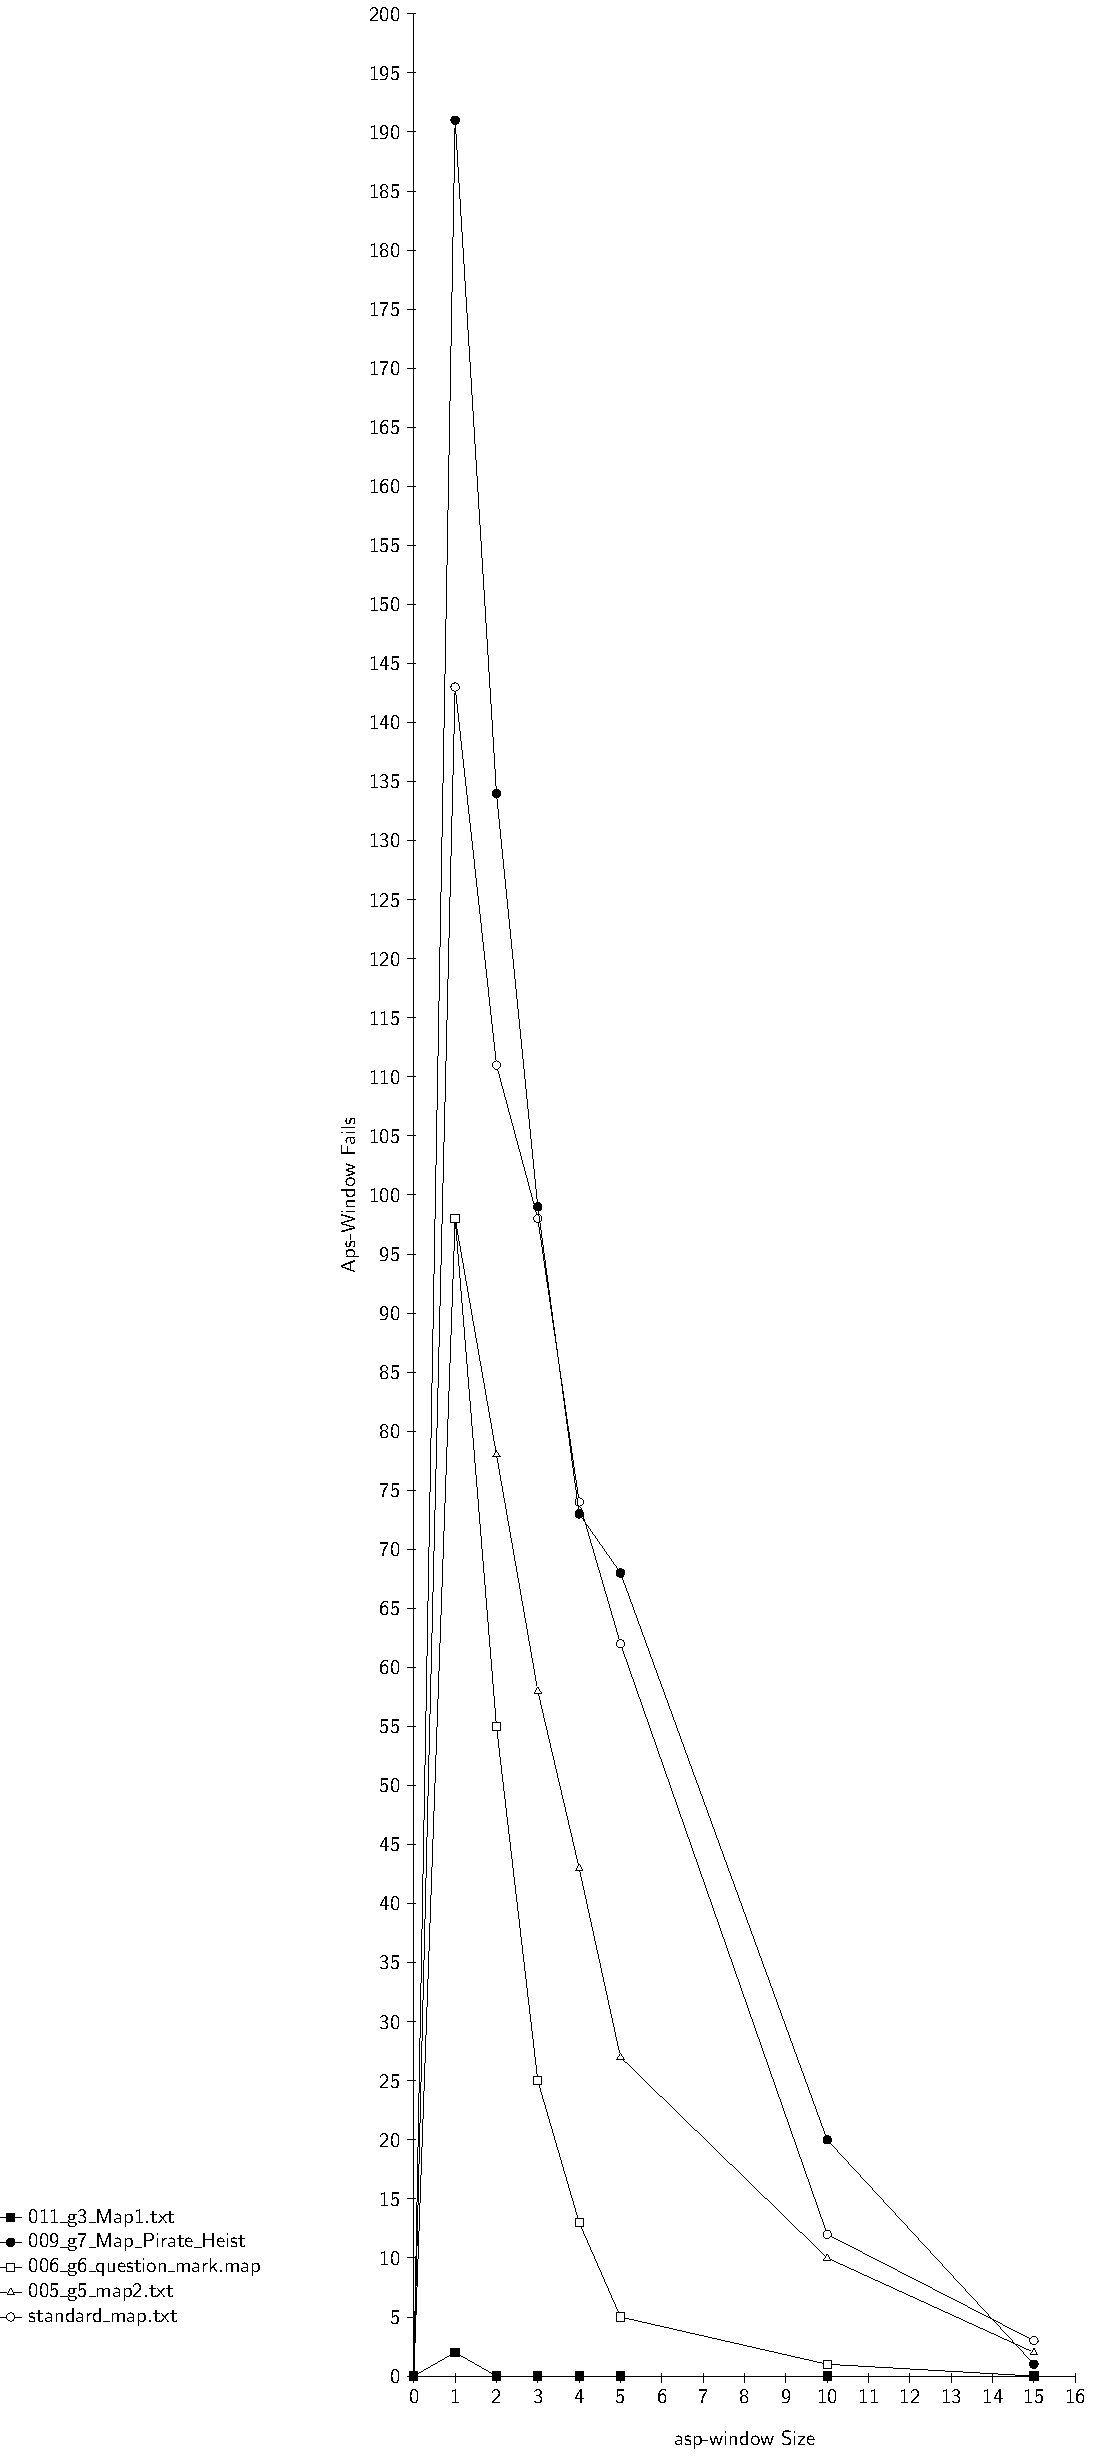
\includegraphics[scale=0.18]{figures/aspFails}
  \end{figure}
\end{frame}

\begin{frame}
\frametitle{Suchfenster Statistiken}
  \begin{figure}
    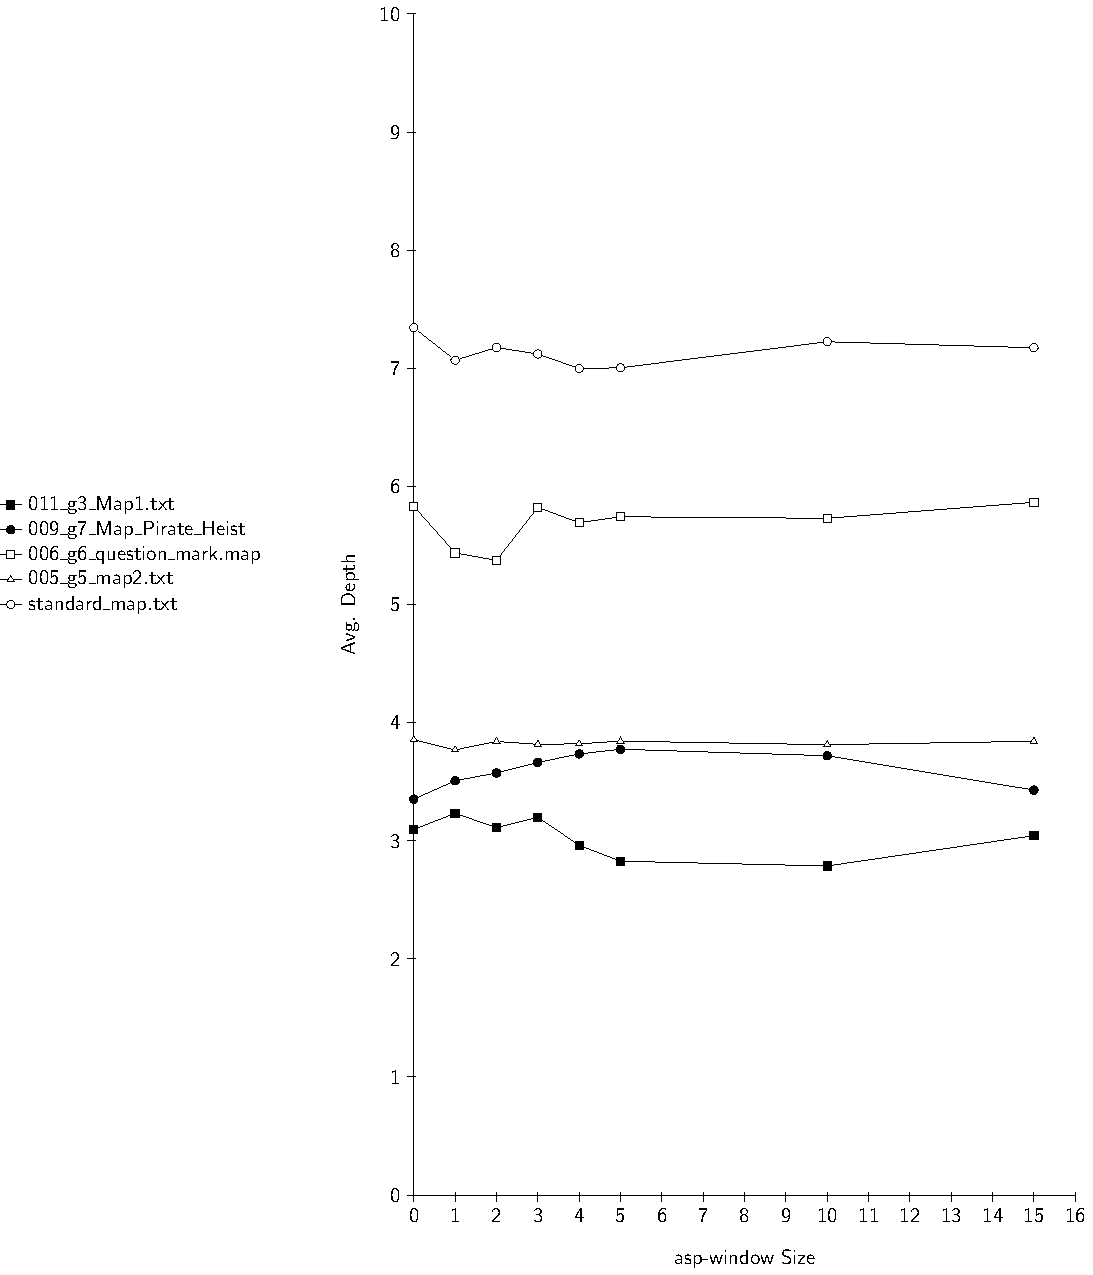
\includegraphics[scale=0.35]{figures/avgDepth}
  \end{figure}
\end{frame}

\appendix
\backupbegin

\begin{frame}
\frametitle{The Stig ablösen?}
  \begin{tabular}{l|l|l|l}
    Game & Ki & Punkte & Duell\\
    \hline
    \multirow{ 2}{*}{2018-06-28\_00:05:01} & Group 3 & 2,150 & \multirow{ 2}{*}{28 : 25}\\
                                         & The Stig & 2,093 \\
     \hline
     \multirow{ 2}{*}{2018-06-27\_18:05:01} & Group 3 & 2,080 & \multirow{ 2}{*}{23 : 32}\\
                                         & The Stig & 2,061 \\
     \hline
     \multirow{ 2}{*}{2018-06-27\_12:05:01} & The Stig & 2,175 & \multirow{ 2}{*}{26 : 21}\\
                                         & Group 3 & 2,101 \\
     \hline
     \multirow{ 2}{*}{2018-06-27\_06:05:01} & Group 3 & 2,133 & \multirow{ 2}{*}{31 : 29}\\
                                         & The Stig & 2,126 \\
     \hline
  
  \end{tabular}
\end{frame}

\begin{frame}
\frametitle{Name}
\begin{huge}
\begin{center}
\textbf{Phteven}
\end{center}
\end{huge}
\end{frame}

\end{document} 